
\subsection{Experimental Setup}

\paragraph{Baselines.} We include LLaMA-3.1-8B-Instruct from Meta \cite{Dubey2024TheL3} and Gemma-3-12B-IT / Gemma-3-27B-IT from Google \cite{Kamath2025Gemma3T} as comparison baselines.  
To evaluate the effectiveness of GRP and PASC-GRPO, we train on the pre-trained Qwen3-4B-Base and Qwen3-8B-Base models from Qwen \cite{Yang2025Qwen3TR}. Detailed training data construction procedures are provided in Appendix~\ref{app:training_data}.

\paragraph{Benchmarks.} For mathematical reasoning, the benchmarks includes GSM8K \cite{Cobbe2021TrainingVT}, MATH500 \cite{Lightman2023LetsVS}, and competition-level benchmarks such as AMC23 \cite{amc23_dataset}, AIME24 \cite{aime24_dataset}, and AIME25 \cite{aime25_dataset}. For code generation, we utilize the widely-used MBPP \cite{Austin2021ProgramSW}, MBPP+ \cite{Liu2023IsYC}, HumanEval \cite{Chen2021EvaluatingLL}, HumanEval+ \cite{Liu2023IsYC}, and the highly challenging LiveCodeBench v5 \cite{Jain2024LiveCodeBenchHA}.

\paragraph{Evaluation Metrics.} For larger datasets (GSM8K, MATH500, and LiveCodeBench), we report the avg@3 accuracy; for other benchmarks, we report the avg@16 accuracy. Considering the extensive derivation required for competition-level mathematics (AIME24, AIME25), we set the \texttt{max\_completion\_tokens} to 32K, while maintaining a limit of 8K for other datasets.

% \paragraph{Training Details} We selected the pre-trained models Qwen3-4B-Base and Qwen3-8B-Base for training. Since our proposed Graph Reasoning Paradigm (GRP) is a novel reasoning paradigm, it is not suitable for models after post-training. Detailed dataset construction, and hyperparameter settings are provided in Appendix~\ref{app:training_details}.

\subsection{Main Results}

\paragraph{Performance Overview.} 
Table~\ref{tab:main_results} reports the performance of our models on mathematical reasoning and code generation benchmarks. 
Both GRP-SFT and PASC-GRPO consistently improve accuracy, demonstrating that the proposed GRP effectively enhances reasoning capabilities.

\paragraph{Impact of GRP-SFT.}
GRP-SFT brings substantial gains in mathematical reasoning. For Qwen3-8B-Base, accuracy improves by 21.52\% on MATH500 and 18.30\% on GSM8K, with a particularly large gain of 36.88\% on the competition-level AMC23 benchmark. Code generation tasks also benefit from GRP-SFT, indicating that the proposed graph-based reasoning paradigm generalizes beyond mathematics.

\paragraph{Effect of PASC-GRPO.}
PASC-GRPO further enhances performance, especially on high-difficulty benchmarks. On AIME24, Qwen3-4B and Qwen3-8B achieve additional gains of 7.23\% and 6.67\% over the SFT stage, respectively. These results suggest that the process-aware reward are effective for multi-step problems.

\paragraph{Comparison with Open-Source LLMs.}
Despite using fewer parameters and training resources, our best model surpasses widely adopted open-source models on competition-level benchmarks.  In particular, it surpasses Gemma-3-27B-IT by over 14\% accuracy on both AIME24 and AIME25, and achieves comparable or better performance on standard math and code benchmarks such as MATH500, AMC23, MBPP+, and HumanEval+. These results highlight the effectiveness of GRP and PASC-GRPO.

\subsection{Ablation Studies}

\begin{table}[htbp]
\centering
\small
\setlength{\tabcolsep}{4pt} % 缩小列间距
\caption{Ablation Experiment Results. Accuracy (\%).}
\label{tab:ablation_combined}
\begin{tabular}{lccc} % 第一列固定宽度，自动换行
\toprule
\textbf{Method} & \textbf{MATH500} & \textbf{AMC23} & \textbf{AIME24} \\
\midrule
Qwen3-8B-Base & 60.08 & 38.12 & 10.00 \\
\midrule
GRP-SFT & 81.60 & 75.00 & 40.00 \\
SFT & 76.45 & 67.80 & 31.50 \\
\midrule
PASC-GRPO & 91.20 & 82.50 & 46.67 \\
GRPO & 88.75 & 79.85 & 43.80 \\
\midrule
w/o Reachability & 87.45 & 79.30 & 40.15 \\
w/o Reach. \& RSR & 83.12 & 76.55 & 35.80 \\
\midrule
w/o SCAE & 84.15 & 76.20 & 32.50 \\
\bottomrule
\end{tabular}
\end{table}


\paragraph{Ablation of GRP and PASC-GRPO.}

We study the effectiveness of GRP and PASC-GRPO.
For SFT, we use the same data as GRP-SFT but replace graph-structured reasoning with standard chain-of-thought.
As shown in Table~\ref{tab:ablation_combined}, this variant performs worse than GRP-SFT on all benchmarks. 

For RL, we compare PASC-GRPO with the original GRPO under identical training settings.
GRPO consistently yields lower performance.
These results show that both graph-structured reasoning and process-aware rewards are essential for strong reasoning performance.

% \input{Tables/ablation_GRP_PASC_GRPO}

\paragraph{Ablation of Reasoning-Length Rewards.}

\begin{figure}[t]
    \centering
    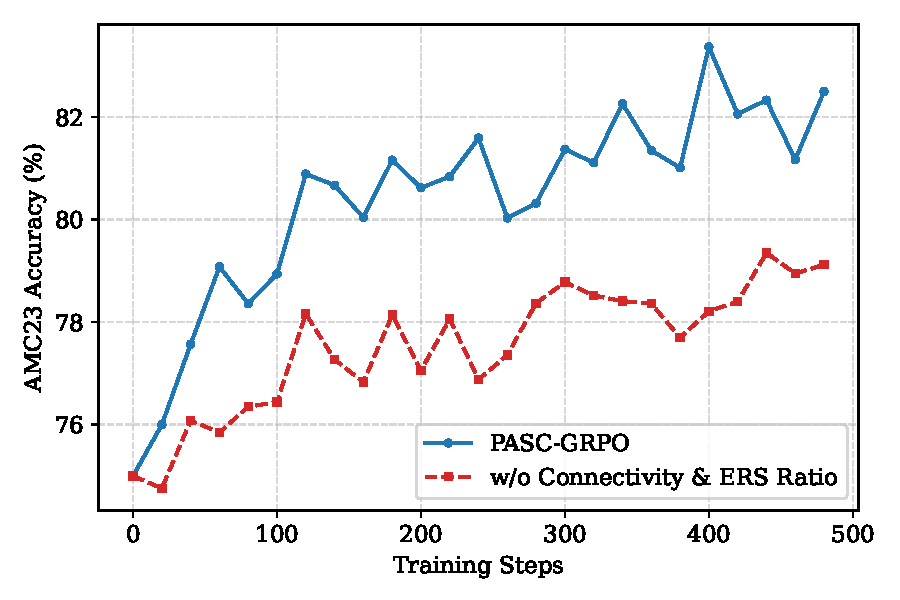
\includegraphics[width=\columnwidth]{Figures/amc23_accuracy_curve.pdf}
    \vspace{0.6em}
    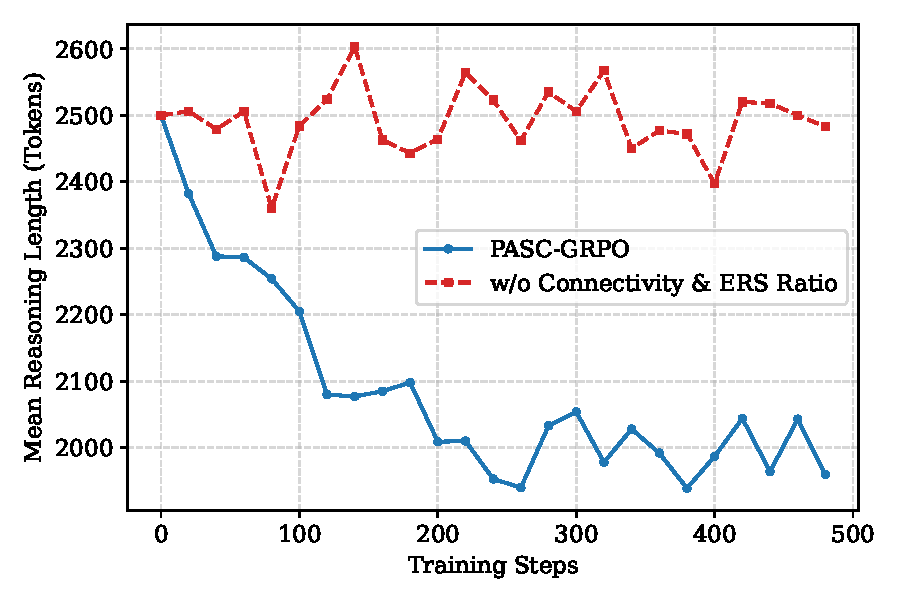
\includegraphics[width=\columnwidth]{Figures/amc23_length_curve.pdf}
    \caption{
    (Top) Accuracy comparison between PASC-GRPO and its variants without connectivity and ERS Ratio rewards on AMC23.
    (Bottom) Corresponding changes in mean reasoning length during training.
    }
    \label{fig:amc23_training_dynamics}
\end{figure}

We remove the connectivity reward and further remove ERS Ratio, starting from the GRP-SFT baseline.
Figure~\ref{fig:amc23_training_dynamics} shows the changes in accuracy and length during training, comparing the cases with and without connectivity and ERS Ratio rewards. For more details on the ablation studies, see Appendix~\ref{app:ablation}.

\paragraph{Ablation of Reasoning process quality rewards.}

Table~\ref{tab:ablation_combined} reports the ablation results of the reachability and reverse search rewards, starting from the GRP-SFT baseline.
Removing the reachability reward leads to a performance drop across all benchmarks.
Further removing the reverse search reward causes a more substantial degradation.
These results indicate that both rewards are critical for guiding effective graph reasoning.

% \input{Tables/ablation_accuracy}

\paragraph{Ablation of SCAE.}

Table~\ref{tab:ablation_combined} shows that using the original GRPO instead of Stratified Clipping Advantage Estimation (SCAE) consistently degrades performance across all benchmarks.
These results suggest that SCAE is crucial for stabilizing the reasoning process and improving accuracy.


% \input{Tables/ablation_SCAE}

\subsection{Discovery}

As shown in Table~\ref{tab:find}, our best model trained from Qwen3-8B-Base matches or surpasses the performance of Qwen3-8B on hard code generation benchmarks. 
Qwen3-8B is a state-of-the-art model distilled using extensive human and computational resources.  
These results highlight the effectiveness of our methods in handling complex reasoning tasks, especially code generation.

\begin{table}[htbp]
\centering
\small
\caption{Performance Comparison on Code Generation}
\label{tab:find}
\begin{tabular}{lccc}
\toprule
\textbf{Model} & \textbf{MBPP} & \textbf{MBPP+} & \textbf{LiveCodeBech}\\
\midrule
qwen3-8B & 76.70 & 65.10 & 57.29 \\
\midrule
qwen3-8B-Base & 73.27 & 61.73 & 29.76 \\
~+ GRP-SFT  & 75.45 & 64.71 & 53.93 \\
~+ PASC-GRPO  & 77.49 & 65.24 & 56.12 \\
\bottomrule
\end{tabular}
\end{table}
